\section{Experiments}
\label{sec:experiments}

We evaluate three training conditions on ALFWorld's 47 unseen test tasks \cite{shridhar2021alfworld}: \textbf{Vanilla} (4{,}358 clean demonstrations), \textbf{TaxEI} (4{,}358 clean + 4{,}671 taxonomy-tagged error trajectories = 9{,}029), and \textbf{Random} (4{,}358 clean + 4{,}671 generic-labeled errors = 9{,}029). All models use Qwen3-8B with LoRA fine-tuning (rank 64, lr $2\times10^{-4}$, 3 epochs). We report results across three seeds (42, 0, 123).

\subsection{Main Results}
\label{sec:main_results}

Table~\ref{tab:main_results} shows three-seed evaluation results. TaxEI degrades directionally ($-8.6$pp vs.\ Vanilla), but the difference is not statistically significant (permutation test, $p{=}0.054$, $N{=}10{,}000$). No TaxEI seed exceeds the Vanilla mean. Random injection shows minimal degradation ($-2.2$pp, $p{>}0.3$).

\begin{table}[t]
\centering
\small
\begin{tabular}{lccccc}
\toprule
\textbf{Method} & \textbf{$N$} & \textbf{s42} & \textbf{s0} & \textbf{s123} & \textbf{Mean$\pm$SD} \\
\midrule
Vanilla & 4{,}358 & 61.7 & 68.1 & 66.0 & 65.3$\pm$3.3 \\
TaxEI   & 9{,}029 & 61.7 & 46.8 & 61.7 & 56.7$\pm$8.6 \\
Random  & 9{,}029 & 66.0 & 55.3 & 68.1 & 63.1$\pm$7.0 \\
\bottomrule
\end{tabular}
\caption{Three-seed clean evaluation on ALFWorld (47 tasks, accuracy \%). TaxEI vs.\ Vanilla: $p{=}0.054$; TaxEI vs.\ Random: $p{=}0.170$; Random vs.\ Vanilla: $p{>}0.3$ (pooled permutation, 10K). Note: TaxEI/Random use $2.1\times$ more training data than Vanilla.}
\label{tab:main_results}
\end{table}

Standard deviations follow a directional ordering: Vanilla (3.3pp) $<$ Random (7.0pp) $<$ TaxEI (8.6pp). However, this pattern is not statistically confirmed at $n{=}3$ (Levene's $p{=}0.085$; $F$-test $p{=}0.252$; bootstrap $P(\text{SD}_\text{TaxEI} > \text{SD}_\text{Vanilla}){=}69\%$).

\subsection{Dose-Response}
\label{sec:dose_response}

To control for data volume, we fix total training size at 4{,}358 and vary the injection ratio (Table~\ref{tab:dose_response}, Figure~\ref{fig:dose_response}). Both methods share a sharp threshold between 10\% and 25\% injection: TaxEI drops from 61.7\% to 48.9\% ($-12.8$pp); Random drops from 68.1\% to 55.3\% ($-12.8$pp). Beyond 25\%, performance plateaus rather than continuing to degrade.

\begin{table}[t]
\centering
\small
\begin{tabular}{lcccc}
\toprule
\textbf{Dose} & \textbf{TaxEI} & \textbf{Random} & \textbf{$\Delta$T} & \textbf{$\Delta$R} \\
\midrule
0\% (Van.)  & 61.7 & 61.7 & ---   & ---   \\
10\%        & 61.7 & 68.1 & 0.0   & +6.4  \\
25\%        & 48.9 & 55.3 & $-$12.8 & $-$6.4  \\
50\%        & 51.1 & 57.4 & $-$10.6 & $-$4.3  \\
\bottomrule
\end{tabular}
\caption{Dose-response ablation (fixed 4{,}358 total, seed=42 only). $\Delta$T/$\Delta$R: change vs.\ vanilla. Both methods share a 12.8pp drop at 10$\to$25\%.}
\label{tab:dose_response}
\end{table}

\begin{figure}[t]
\centering
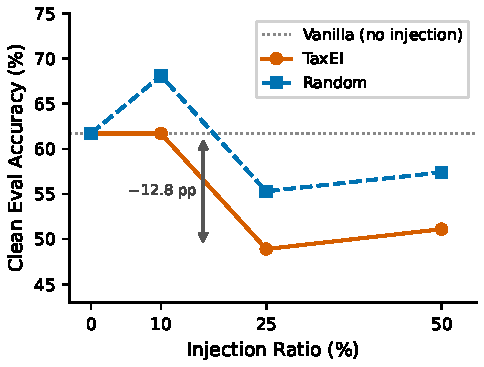
\includegraphics[width=\columnwidth]{figures/paper/fig1_dose_response.pdf}
\caption{Dose-response: accuracy vs.\ injection ratio. Both TaxEI and Random share a 12.8pp collapse at 10$\to$25\%. Single seed (seed=42).}
\label{fig:dose_response}
\end{figure}

At 10\% injection, TaxEI is task-identical to Vanilla (same success/failure on every task), while Random shows a +6.4pp augmentation effect. This suggests the model absorbs sub-threshold random noise as data augmentation but ignores taxonomy-tagged errors entirely at low doses.

\subsection{Task-Type Vulnerability}
\label{sec:task_vulnerability}

The TaxEI--Random gap is not uniform across task types. Three-seed averages reveal that two of six task types drive the aggregate difference: \texttt{pick\_cool} (TaxEI$-$Random $= -19.0$pp) and \texttt{pick\_two\_obj} ($-14.3$pp). The remaining four types show gaps $\leq$4.2pp, with \texttt{pick\_heat} and \texttt{look\_at\_obj} at exactly 0pp. This concentration suggests taxonomy-guided errors interact with specific action-sequence structures rather than causing uniform degradation.

\subsection{Recovery Evaluation}
\label{sec:recovery}

We test whether error-trained models recover from injected errors at inference time using round-robin operator injection across 47 tasks (seed=42). TaxEI achieves 59.6\% recovery (vs.\ Vanilla 61.7\%, Random 63.8\%)---no improvement over the clean baseline. Error detection rate is 0\% for all methods: no model produces explicit error acknowledgment before attempting recovery.
